\section{Results}
\label{sec:results}

\subsection{What the released files contain}
\label{sec:files}
Table~\ref{tab:artefacts} compares the two classes of each corpus on presentation, scheme-type and structure properties. Every corpus differs between its classes in at least one presentation property. In PhiUSIIL every legitimate string has the form \texttt{https://www.}\emph{domain}, with no path and no trailing slash, while fewer than half of the phishing strings use \texttt{https} or \texttt{www.}. In PT-Alexa no legitimate string carries a scheme and every phishing string does. In both corpora no legitimate URL has a path, so the popularity-list design couples a presentation contrast with a sampling contrast. The HTML-escaped ampersand occurs in at most \AmpLegitMaxOther\% of the legitimate strings of six corpora; Kaggle-MU is the exception (1.7\% of legitimate and 3.1\% of phishing strings). Its presence points to the way phishing feeds were exported. ISCX-URL2016 shows the reverse \texttt{www.} pattern: the prefix is almost absent from legitimate strings and present in 42.2\% of phishing strings.

Table~\ref{tab:overlap} lists hygiene problems that exist before any model is trained. Ebbu2017 contains \DupEbbu{} exact duplicate rows, \DupPctEbbu\% of the file (\DupLegitEbbu{} legitimate and \DupPhishEbbu{} phishing). Canonicalisation collapses a further \CanonDupPhishStorm{} rows in PhishStorm and \CanonDupKaggleMU{} in Kaggle-MU. All experiments therefore run on canonical-unique strings, so that no canonical string can occur on both sides of a split.

Kaggle-MU shows label inconsistencies on a scale that changes how its results should be read. It has \CanonConfKaggleMU{} canonical strings with both labels and \MixedKaggleMU{} registered domains with URLs of both classes. The registered domain with the most phishing URLs is \texttt{\LargestPhishKaggleMU}, with \LargestPhishPctKaggleMU\% of the phishing class, and \TopKKaggleMU\% of its phishing rows sit on a registered domain from the Alexa top 1,000, against \TopKMinOther\% to \TopKMaxOther\% in the other corpora; in \TopKMaxOtherCorpus{} most of these are phishing pages on a large platform (\texttt{\LargestPhishPTAlexa}). Two corpora share a URL when their canonical-unique strings are identical. Kaggle-MU shares \XSharedKaggleMUPhishStorm{} canonical URLs with PhishStorm; \XConfKaggleMUPhishStorm{} of them carry opposite labels, and in \XConfAPKaggleMUPhishStorm{} of these Kaggle-MU calls phishing a URL that PhishStorm calls legitimate. Kaggle-MU also contains \XSharedISCXURLKaggleMU{} canonical URLs of ISCX-URL2016, \ISCXInKagglePct\% of that corpus and every one of its legitimate URLs, so results on the two are not independent evidence.

Registered-domain overlap under random splits is large. The share of test URLs whose registered domain also occurs in training ranges from \SeenPhiUSIIL\% (PhiUSIIL) to \SeenISCXURL\% (ISCX-URL2016). ISCX-URL2016 draws its \UniqISCXURL{} unique URLs from only \RegLegitISCXURL{} legitimate registered domains, against \RegPhishISCXURL{} phishing ones.

\begin{table}[tp]
\centering
\caption{Presentation, scheme-type and structure properties by class (L: legitimate, P: phishing), computed on the exact-de-duplicated files. Columns give the percentage of URLs with the property, except the last pair, which gives the median canonical length in characters.}
\label{tab:artefacts}
\footnotesize
\setlength{\tabcolsep}{3pt}
\begin{adjustbox}{max width=\linewidth}
\begin{tabular}{@{}l*{14}{r}@{}}
\toprule
 & \multicolumn{2}{c}{Scheme} & \multicolumn{2}{c}{www.} & \multicolumn{2}{c}{Trailing /} & \multicolumn{2}{c}{\texttt{\&amp;}} & \multicolumn{2}{c}{https} & \multicolumn{2}{c}{Has path} & \multicolumn{2}{c}{Length} \\
\cmidrule(lr){2-3}\cmidrule(lr){4-5}\cmidrule(lr){6-7}\cmidrule(lr){8-9}\cmidrule(lr){10-11}\cmidrule(lr){12-13}\cmidrule(lr){14-15}
Corpus & L & P & L & P & L & P & L & P & L & P & L & P & L & P \\
\midrule
Ebbu2017 & 100.0 & 99.7 & 58.8 & 26.1 & 26.9 & 39.8 & 0.0 & 8.5 & 36.1 & 2.0 & 95.0 & 97.8 & 45 & 50 \\
PhishStorm & 100.0 & 100.0 & 68.0 & 34.5 & 35.8 & 35.5 & 0.0 & 8.0 & 2.2 & 1.4 & 99.7 & 99.8 & 34 & 53 \\
ISCX-URL2016 & 100.0 & 99.8 & 0.4 & 42.2 & 19.5 & 38.9 & 0.0 & 8.5 & 5.5 & 1.7 & 99.7 & 96.2 & 94 & 59 \\
PT-Alexa & 0.0 & 100.0 & 0.1 & 12.8 & 0.0 & 27.2 & 0.0 & 11.3 & 0.0 & 47.1 & 0.0 & 83.1 & 12 & 52 \\
Hannousse2021 & 100.0 & 100.0 & 66.8 & 20.5 & 45.3 & 29.7 & 0.0 & 4.2 & 44.5 & 33.3 & 61.3 & 80.2 & 31 & 46 \\
PhiUSIIL & 100.0 & 100.0 & 100.0 & 41.5 & 0.0 & 36.3 & 0.0 & 1.2 & 100.0 & 48.6 & 0.0 & 27.1 & 15 & 25 \\
Kaggle-MU & 8.3 & 26.4 & 3.1 & 38.7 & 26.0 & 27.4 & 1.7 & 3.1 & 0.5 & 7.4 & 87.8 & 74.6 & 45 & 31 \\
\bottomrule
\end{tabular}
\end{adjustbox}
\end{table}

\begin{table}[tp]
\centering
\caption{Duplicates, collisions and domain structure inside each corpus. Exact dup.: repeated raw strings with the same label. Raw conflict: rows whose raw string carries both labels. Canon.\ dup.: further rows that collapse after canonicalisation; Canon.\ conflict: canonical strings with both labels. Reg.\ L/P: registered domains in the legitimate and phishing class (PSL private suffixes treated as public). Mixed: registered domains with URLs of both classes. Seen: share of test URLs in a random 80/20 split whose registered domain occurs in training (mean over 10 seeds, \%).}
\label{tab:overlap}
\footnotesize
\begin{adjustbox}{max width=\linewidth}
\begin{tabular}{@{}lrrrrrrrr@{}}
\toprule
Corpus & Exact dup. & Raw conflict & Canon.\ dup. & Canon.\ conflict & Reg.\ L & Reg.\ P & Mixed & Seen \\
\midrule
Ebbu2017 & 18,812 & 0 & 3,042 & 0 & 12,735 & 8,930 & 16 & 67.8 \\
PhishStorm & 0 & 0 & 10,420 & 0 & 17,340 & 13,756 & 52 & 67.3 \\
ISCX-URL2016 & 9 & 0 & 583 & 0 & 307 & 4,154 & 1 & 90.5 \\
PT-Alexa & 7 & 0 & 2,529 & 0 & 15,553 & 6,253 & 81 & 29.0 \\
Hannousse2021 & 1 & 0 & 359 & 0 & 4,103 & 3,174 & 17 & 40.7 \\
PhiUSIIL & 425 & 0 & 3,621 & 43 & 132,186 & 65,629 & 106 & 15.3 \\
Kaggle-MU & 42 & 12 & 9,097 & 3,971 & 111,801 & 46,492 & 4,313 & 53.1 \\
\bottomrule
\end{tabular}
\end{adjustbox}
\end{table}


\subsection{What formatting alone predicts}
\label{sec:probe}
Figure~\ref{fig:within} and Table~\ref{tab:within_random} give the within-corpus results under the random split. The presentation probe sees five binary flags and none of the characters of host, path or query. It reaches an MCC of \WPTAlexaRandomPresentation{} on PT-Alexa and between \PresMinMCC{} (\PresMinCorpus) and \WPhiUSIILRandomPresentation{} (PhiUSIIL) on the six published corpora. Adding the scheme-type flag lifts PhiUSIIL to \WPhiUSIILRandomPresentationHttps{} and Ebbu2017 from \WEbbuRandomPresentation{} to \WEbbuRandomPresentationHttps{}; on the other corpora it changes the probe by less than 0.04.

These values describe how separable a corpus is by formatting. They are not bounds on how much of a content model's score comes from formatting, because a model that reads host and path can recover the same information in other ways; the canonicalisation experiment in Section~\ref{sec:canon} measures that dependence directly.

The probe ablation (Table~\ref{tab:probe}) shows which flag carries the signal. On PT-Alexa the scheme flag alone does: without it the probe falls from \ProbePTAlexaAll{} to \ProbePTAlexaDropHasScheme{}, and removing any other flag changes nothing. On the six published corpora the \texttt{www.} flag carries the largest share; removing it lowers the probe on PhiUSIIL from \ProbePhiUSIILAll{} to \ProbePhiUSIILDropHasWww{} and on Hannousse2021 from \ProbeHannousseAll{} to \ProbeHannousseDropHasWww.

Homepage sampling can masquerade as a presentation signal, because a homepage has no path and therefore no trailing slash after one. Two subsets remove this confound by sampling both classes at the same granularity: the path subset keeps only URLs with a path, and the homepage subset only URLs without one. On Ebbu2017, PhishStorm and ISCX-URL2016 it stays within 0.01 of the full probe (\ProbeEbbuPathSubset, \ProbePhishStormPathSubset{} and \ProbeISCXURLPathSubset), on Hannousse2021 it falls to \ProbeHannoussePathSubset, and on Kaggle-MU it rises to \ProbeKaggleMUPathSubset. On those five corpora the presentation signal is therefore not a by-product of homepage sampling. On PT-Alexa and PhiUSIIL no legitimate URL has a path, so only the homepage subset applies (Table~\ref{tab:controls}): with \HomeNPhiUSIIL{} legitimate and phishing homepages, PhiUSIIL still gives a probe MCC of \HomePhiUSIILPresentationHttps{} with the scheme-type flag, a raw-string MCC of \HomePhiUSIILCharRaw{} and a canonical MCC of \HomePhiUSIILCharCanon; PT-Alexa gives \HomePTAlexaPresentationHttps, \HomePTAlexaCharRaw{} and \HomePTAlexaCharCanon. The formatting contrast of these two corpora thus survives when both classes are homepages.

\begin{figure}[t]
\centering
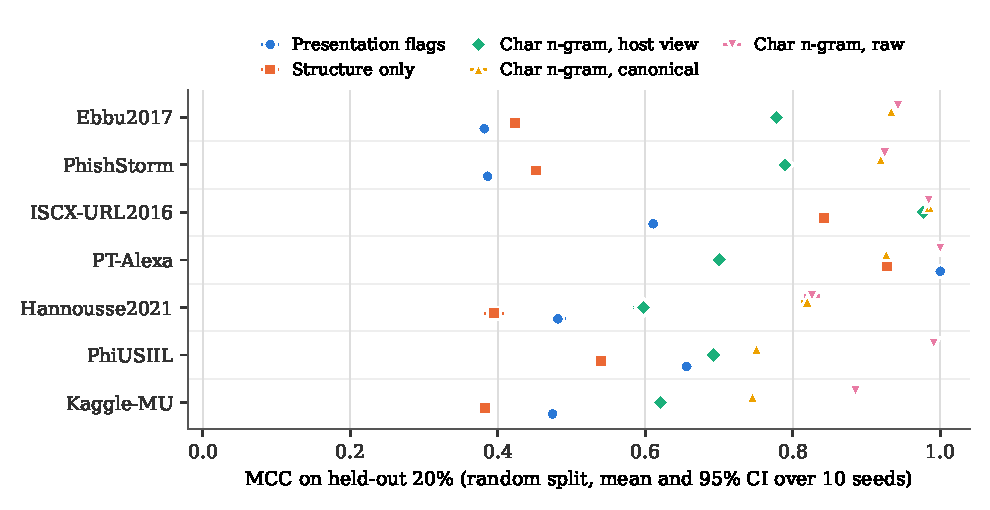
\includegraphics[width=\linewidth]{figures/fig_within.pdf}
\caption{Within-corpus MCC under a stratified random split (mean over 10 seeds; horizontal bars are 95\% CIs and are often narrower than the markers). Colour and marker shape both identify the detector. The lexical and presentation-plus-https detectors are omitted for legibility and appear in Table~\ref{tab:within_random}. The gap between the raw-string marker and the canonical marker measures dependence on presentation features; the gap between canonical and host-view markers measures dependence on path information, which includes the homepage-sampling artefact.}
\label{fig:within}
\end{figure}

\begin{table}[tp]
\centering
\caption{Within-corpus MCC (mean\,$\pm$\,95\% CI half-width over 10 repeated splits), stratified random 80/20 split. Pres.: the five presentation flags; Pres.+https adds the scheme-type flag.}
\label{tab:within_random}
\footnotesize
\setlength{\tabcolsep}{3pt}
\begin{adjustbox}{max width=\linewidth}
\begin{tabular}{@{}lrrrrrrr@{}}
\toprule
Corpus & Pres. & Pres.+https & Structure & Lexical & Char raw & Char canon. & Char host \\
\midrule
Ebbu2017 & 0.382\,$\pm$\,0.003 & 0.529\,$\pm$\,0.004 & 0.424\,$\pm$\,0.004 & 0.782\,$\pm$\,0.004 & 0.943\,$\pm$\,0.002 & 0.933\,$\pm$\,0.003 & 0.778\,$\pm$\,0.004 \\
PhishStorm & 0.386\,$\pm$\,0.004 & 0.386\,$\pm$\,0.003 & 0.452\,$\pm$\,0.008 & 0.752\,$\pm$\,0.003 & 0.925\,$\pm$\,0.002 & 0.919\,$\pm$\,0.002 & 0.789\,$\pm$\,0.004 \\
ISCX-URL2016 & 0.611\,$\pm$\,0.006 & 0.617\,$\pm$\,0.007 & 0.842\,$\pm$\,0.004 & 0.990\,$\pm$\,0.002 & 0.984\,$\pm$\,0.002 & 0.985\,$\pm$\,0.002 & 0.977\,$\pm$\,0.002 \\
PT-Alexa & 1.000\,$\pm$\,0.000 & 1.000\,$\pm$\,0.000 & 0.928\,$\pm$\,0.003 & 0.953\,$\pm$\,0.003 & 1.000\,$\pm$\,0.000 & 0.927\,$\pm$\,0.004 & 0.701\,$\pm$\,0.009 \\
Hannousse2021 & 0.482\,$\pm$\,0.010 & 0.482\,$\pm$\,0.010 & 0.395\,$\pm$\,0.013 & 0.738\,$\pm$\,0.006 & 0.826\,$\pm$\,0.011 & 0.820\,$\pm$\,0.008 & 0.598\,$\pm$\,0.014 \\
PhiUSIIL & 0.656\,$\pm$\,0.003 & 0.985\,$\pm$\,0.001 & 0.540\,$\pm$\,0.007 & 0.701\,$\pm$\,0.004 & 0.991\,$\pm$\,0.001 & 0.751\,$\pm$\,0.004 & 0.693\,$\pm$\,0.005 \\
Kaggle-MU & 0.474\,$\pm$\,0.004 & 0.513\,$\pm$\,0.005 & 0.383\,$\pm$\,0.007 & 0.564\,$\pm$\,0.008 & 0.885\,$\pm$\,0.002 & 0.745\,$\pm$\,0.004 & 0.621\,$\pm$\,0.007 \\
\bottomrule
\end{tabular}
\end{adjustbox}
\end{table}

\begin{table}[tp]
\centering
\caption{Presentation-probe ablation (MCC, random split, mean over 10 seeds). $-$X: probe without flag X (scheme: explicit scheme; slash: string ends in a slash; case: upper-case letter in the host). Path subset: probe trained and tested only on URLs that have a path, which removes the homepage-sampling contrast; --: fewer than 500 such URLs in one class. Last column: legitimate/phishing URLs with a path.}
\label{tab:probe}
\footnotesize
\setlength{\tabcolsep}{3pt}
\begin{adjustbox}{max width=\linewidth}
\begin{tabular}{@{}lrrrrrrrrr@{}}
\toprule
Corpus & All five & +https & $-$scheme & $-$www. & $-$slash & $-$\texttt{\&amp;} & $-$case & Path subset & $n$ with path (L/P) \\
\midrule
Ebbu2017 & 0.382 & 0.529 & 0.382 & 0.212 & 0.382 & 0.359 & 0.381 & 0.379 & 23,779/21,306 \\
PhishStorm & 0.386 & 0.386 & 0.386 & 0.228 & 0.386 & 0.359 & 0.386 & 0.383 & 24,920/24,941 \\
ISCX-URL2016 & 0.611 & 0.617 & 0.611 & 0.251 & 0.611 & 0.579 & 0.611 & 0.619 & 24,914/9,366 \\
PT-Alexa & 1.000 & 1.000 & 0.529 & 1.000 & 1.000 & 1.000 & 1.000 & -- & 0/11,024 \\
Hannousse2021 & 0.482 & 0.482 & 0.482 & 0.164 & 0.482 & 0.471 & 0.482 & 0.426 & 3,501/4,279 \\
PhiUSIIL & 0.656 & 0.985 & 0.656 & 0.475 & 0.640 & 0.654 & 0.656 & -- & 0/6,743 \\
Kaggle-MU & 0.474 & 0.513 & 0.454 & 0.176 & 0.474 & 0.474 & 0.474 & 0.609 & 21,949/18,349 \\
\bottomrule
\end{tabular}
\end{adjustbox}
\end{table}


\subsection{Removing presentation features}
\label{sec:canon}
Canonicalisation lowers the character model substantially on three corpora (Table~\ref{tab:tests}). On PhiUSIIL the MCC falls from \WPhiUSIILRandomCharRaw{} to \WPhiUSIILRandomCharCanon, a paired drop of \DRawVsCanonPhiUSIIL{} (ROC-AUC drop \DARawVsCanonPhiUSIIL); on Kaggle-MU it falls by \DRawVsCanonKaggleMU{} and on PT-Alexa by \DRawVsCanonPTAlexa. On the four other corpora the mean drop is below 0.01. Its corrected 95\% interval is widest on Hannousse2021 (\DLoRawVsCanonHannousse{} to \DHiRawVsCanonHannousse), so these data cannot exclude a formatting dependence of a few hundredths there, but they exclude one of the size seen on PhiUSIIL and Kaggle-MU. These four corpora have moderate presentation probes, yet their character models do not rely on the formatting flags.

Further controls test competing explanations (Tables~\ref{tab:controls} and~\ref{tab:controls2}). Kaggle-MU's drop could reflect its label inconsistencies rather than formatting, because many of its contested rows are scheme-less. On Kaggle-MU-clean, which removes the \KCleanNMixedRows{} rows of registered domains with both labels and the phishing rows that another corpus labels legitimate, the raw-string model reaches \KCleanCharRaw{} and the canonical model \KCleanCharCanon. That rule misses a second group of doubtful rows: \KCleanBareWwwPct\% of the remaining phishing class starts with a bare \texttt{www.}, mostly content pages of small software, publishing and research sites (largest registered domains \KWwwTopDomains), and only \KWwwKwShare\% of these rows contain a brand or credential keyword, against \KOtherKwShare\% of the other phishing rows. They look like a list of benign pages that received the phishing label. Without them the probe falls to \KCleanTwoPresentationHttps, while the raw-string model reaches \KCleanTwoCharRaw{} and the canonical model \KCleanTwoCharCanon, a drop of \KCleanTwoDrop. Kaggle-MU's character model therefore depends on formatting beyond these rows, but in a collection that mixes sources this way we cannot say how much of the dependence is a phishing feed's convention and how much marks the source a row came from. Among Kaggle-MU homepages the contrast is extreme: the probe reaches \HomeKaggleMUPresentationHttps, the raw-string model \HomeKaggleMUCharRaw{} and the canonical model \HomeKaggleMUCharCanon, because \HomeSlashLegitKaggleMU\% of legitimate homepage strings end in a slash against \HomeSlashPhishKaggleMU\% of phishing ones.

Adding a single token for an explicit \texttt{https} scheme to the canonical string raises PhiUSIIL from \WPhiUSIILRandomCharCanon{} to \CanonHttpsPhiUSIIL, so most of its formatting dependence is carried by the scheme type. This is not evidence of a server property: every legitimate PhiUSIIL string carries the same \texttt{https://www.} prefix, a curator's template. On the other corpora the token changes the canonical model by between \CanonHttpsGainPhishStorm{} and \CanonHttpsGainPTAlexa{} MCC. In the PhishTank dump, where submission times allow a time split, training on phishing URLs submitted up to 2019 (\TimeTrainHttps\% with \texttt{https}) and testing on 2020 submissions (\TimeTestHttps\%) gives the canonical model \TimeCharCanon{} against \TimeRandCharCanon{} for a split of the same size drawn from all years, and \TimeCharCanonHttps{} against \TimeRandCharCanonHttps{} with the scheme token, a loss of \TimeGapCharCanon{} and \TimeGapCharCanonHttps{} MCC when the phishing class of the test set is newer than that of the training set and the legitimate class is held fixed. The raw-string model and the probe stay at \TimeCharRaw{} and \TimePresentationHttps{}, because the scheme convention that separates PT-Alexa does not change over time.

Table~\ref{tab:precision} converts the test error rates into the precision a detector would reach at 1\% and 0.1\% phishing prevalence. At the default threshold of 0.5 the canonical model stays at or below \PrecOneEbbuRandomCharCanon{} at 1\% prevalence on every published corpus except ISCX-URL2016 (\PrecOneISCXURLRandomCharCanon{} random, \PrecOneISCXURLDomainCharCanon{} grouped). The raw-string model on PhiUSIIL is the exception that formatting allows: it made no false positive in any of the 10 seeds, each with \NLegTestPhiUSIIL{} legitimate test URLs, so a conservative per-seed 95\% upper bound on its false-positive rate is about 3 in \NLegTestPhiUSIIL. A threshold chosen on validation data for a false-positive rate of at most 0.1\% keeps that rate on the test part of the same corpus: the realised rate of the canonical model lies between \VFprHannousseCharCanon\% (Hannousse2021) and \VFprEbbuCharCanon\% (Ebbu2017). At 1\% prevalence this gives the canonical model a precision of \VPrecOneEbbuCharCanon{} on Ebbu2017, \VPrecOnePhishStormCharCanon{} on PhishStorm and \VPrecOneKaggleMUCharCanon{} on Kaggle-MU, at true-positive rates of \VTprEbbuCharCanon, \VTprPhishStormCharCanon{} and \VTprKaggleMUCharCanon. At 0.1\% prevalence no published corpus gives the canonical model a precision above \VPrecTenthISCXURLCharCanon, so most alarms would still be false. The low rate is reached at a cost in recall that the balanced MCC hides; on Hannousse2021 the true-positive rate falls to \VTprHannousseCharCanon, and its \VNZeroHannousseCharCanon{} legitimate test URLs over ten seeds yield only \VFPHannousseCharCanon{} false positives, so its rates are imprecise.

\begin{table}[tp]
\centering
\caption{Test-set error rates and the precision a within-corpus detector would reach at 1\% and 0.1\% phishing prevalence (random split, 10 seeds). Validation threshold: 20\% of the training part is held out, the model is fitted on the rest, and the threshold with the highest validation true-positive rate at a validation false-positive rate of at most 0.1\% is applied to the test part; FPR and TPR are the realised test rates. @0.5: the model fitted on the full training part at threshold 0.5. Rates are pooled over seeds before precision is computed.}
\label{tab:precision}
\footnotesize
\setlength{\tabcolsep}{3pt}
\begin{adjustbox}{max width=\linewidth}
\begin{tabular}{@{}lrrrrrrrrrr@{}}
\toprule
 & \multicolumn{5}{c}{Char raw} & \multicolumn{5}{c}{Char canon.} \\
\cmidrule(lr){2-6}\cmidrule(lr){7-11}
 & \multicolumn{4}{c}{Validation threshold} & @0.5 & \multicolumn{4}{c}{Validation threshold} & @0.5 \\
\cmidrule(lr){2-5}\cmidrule(lr){6-6}\cmidrule(lr){7-10}\cmidrule(lr){11-11}
Corpus & FPR (\%) & TPR & Prec.\ 1\% & Prec.\ 0.1\% & Prec.\ 1\% & FPR (\%) & TPR & Prec.\ 1\% & Prec.\ 0.1\% & Prec.\ 1\% \\
\midrule
Ebbu2017 & 0.14 & 0.766 & 0.850 & 0.360 & 0.277 & 0.16 & 0.730 & 0.820 & 0.311 & 0.293 \\
PhishStorm & 0.12 & 0.753 & 0.862 & 0.382 & 0.279 & 0.11 & 0.712 & 0.869 & 0.398 & 0.265 \\
ISCX-URL2016 & 0.10 & 0.974 & 0.908 & 0.494 & 0.906 & 0.11 & 0.947 & 0.900 & 0.472 & 0.847 \\
PT-Alexa & 0.00 & 1.000 & 1.000 & 1.000 & 1.000 & 0.11 & 0.779 & 0.879 & 0.420 & 0.611 \\
Hannousse2021 & 0.07 & 0.343 & 0.832 & 0.329 & 0.101 & 0.05 & 0.206 & 0.798 & 0.282 & 0.128 \\
PhiUSIIL & 0.10 & 0.995 & 0.913 & 0.509 & 1.000 & 0.13 & 0.585 & 0.820 & 0.311 & 0.128 \\
Kaggle-MU & 0.15 & 0.199 & 0.570 & 0.116 & 0.153 & 0.11 & 0.127 & 0.548 & 0.107 & 0.055 \\
\bottomrule
\end{tabular}
\end{adjustbox}
\end{table}

\begin{table}[tp]
\centering
\caption{Controls (MCC, random split, mean over 10 seeds). Homepage subset: only URLs without a path, so that both classes are sampled at the same granularity; $n$: legitimate and phishing homepages in the capped sample; --: fewer than 500 such URLs in one class. Full corpus: the canonical model of Table~\ref{tab:within_random} and the same model with a token for an explicit \texttt{https} scheme prepended to the canonical string.}
\label{tab:controls}
\footnotesize
\begin{adjustbox}{max width=\linewidth}
\begin{tabular}{@{}lrrrrrr@{}}
\toprule
 & \multicolumn{4}{c}{Homepage subset (no path in either class)} & \multicolumn{2}{c}{Full corpus} \\
\cmidrule(lr){2-5}\cmidrule(lr){6-7}
Corpus & $n$ (L/P) & Pres.+https & Char raw & Char canon. & Char canon. & Canon.+https \\
\midrule
Ebbu2017 & 1,248/509 & 0.464 & 0.779 & 0.721 & 0.933 & 0.942 \\
PhishStorm & 90/60 & -- & -- & -- & 0.919 & 0.919 \\
ISCX-URL2016 & 81/370 & -- & -- & -- & 0.985 & 0.987 \\
PT-Alexa & 15,753/2,193 & 1.000 & 0.999 & 0.698 & 0.927 & 0.947 \\
Hannousse2021 & 2,213/1,077 & 0.556 & 0.783 & 0.708 & 0.820 & 0.828 \\
PhiUSIIL & 25,000/18,433 & 0.996 & 0.991 & 0.709 & 0.751 & 0.967 \\
Kaggle-MU & 3,033/6,607 & 0.933 & 0.925 & 0.503 & 0.745 & 0.751 \\
\bottomrule
\end{tabular}
\end{adjustbox}
\end{table}

\begin{table}[tp]
\centering
\caption{Kaggle-MU subsets and a time split (MCC, mean over seeds). Kaggle-MU rows: random split, 10 seeds, at most 25,000 URLs per class; $n$: legitimate/phishing rows before the cap. Kaggle-MU-clean drops registered domains with both labels and phishing URLs that another corpus labels legitimate; the next row also drops phishing URLs that start with a bare \texttt{www.} (the rule also removes phishing URLs on Alexa top-1,000 domains, but none remain after the first rule). PT-Alexa rows: 3 seeds; $n$: phishing URLs for training/testing, with as many legitimate URLs drawn at random; the time split trains on phishing URLs submitted up to 2019 and tests on 2020 submissions, the matched control draws the same numbers from all years.}
\label{tab:controls2}
\footnotesize
\setlength{\tabcolsep}{3pt}
\begin{adjustbox}{max width=\linewidth}
\begin{tabular}{@{}>{\raggedright\arraybackslash}p{4.2cm}rrrrr@{}}
\toprule
Control & $n$ & Pres.+https & Char raw & Char canon. & Canon.+https \\
\midrule
Kaggle-MU, full & 509,092 in all & 0.513 & 0.885 & 0.745 & -- \\
Kaggle-MU-clean & 312,932/52,034 & 0.474 & 0.904 & 0.739 & -- \\
Kaggle-MU-clean without bare-\texttt{www.} phishing & 312,932/37,968 & 0.351 & 0.904 & 0.763 & -- \\
\midrule
PT-Alexa, random years (matched) & 2,373/5,000 & 1.000 & 1.000 & 0.898 & 0.924 \\
PT-Alexa, train $\le$2019, test 2020 & 2,373/5,000 & 1.000 & 1.000 & 0.865 & 0.897 \\
\bottomrule
\end{tabular}
\end{adjustbox}
\end{table}


\begin{table}[tp]
\centering
\caption{Differences paired by seed over 10 repeated splits: mean MCC and ROC-AUC difference with a 95\% interval that uses the variance correction of \citet{nadeau2003}, and a Holm-adjusted $p$-value from the corrected resampled $t$-test across the seven corpora of each comparison. For the random-versus-grouped comparisons the two settings share the sample of a seed but not the split. Differences smaller than 0.0005 in absolute value print as $+$0.000; small $p$-values for such rows reflect very small seed variance, not a material effect.}
\label{tab:tests}
\footnotesize
\scriptsize
\setlength{\tabcolsep}{3pt}
\begin{adjustbox}{max width=\linewidth}
\begin{tabular}{@{}lrrrr@{}}
\toprule
Comparison and corpus & $\Delta$MCC [95\% CI] & $p_\mathrm{Holm}$ & $\Delta$AUC [95\% CI] & $p_\mathrm{Holm}$ \\
\midrule
\multicolumn{5}{@{}l}{\emph{Char raw $-$ canonical (random split)}} \\
\quad Ebbu2017 & +0.009 [+0.004, +0.014] & 0.012 & +0.001 [+0.001, +0.002] & 0.006 \\
\quad PhishStorm & +0.006 [+0.002, +0.009] & 0.017 & +0.001 [+0.000, +0.001] & 0.008 \\
\quad ISCX-URL2016 & $-$0.001 [$-$0.005, +0.003] & 1.000 & +0.000 [+0.000, +0.000] & 0.008 \\
\quad PT-Alexa & +0.073 [+0.066, +0.080] & $<$0.001 & +0.010 [+0.008, +0.012] & $<$0.001 \\
\quad Hannousse2021 & +0.006 [$-$0.014, +0.027] & 1.000 & +0.005 [+0.001, +0.010] & 0.028 \\
\quad PhiUSIIL & +0.240 [+0.234, +0.246] & $<$0.001 & +0.070 [+0.066, +0.073] & $<$0.001 \\
\quad Kaggle-MU & +0.140 [+0.133, +0.147] & $<$0.001 & +0.038 [+0.037, +0.039] & $<$0.001 \\
\multicolumn{5}{@{}l}{\emph{Char raw $-$ host view (random split)}} \\
\quad Ebbu2017 & +0.165 [+0.156, +0.173] & $<$0.001 & +0.040 [+0.037, +0.042] & $<$0.001 \\
\quad PhishStorm & +0.136 [+0.129, +0.143] & $<$0.001 & +0.033 [+0.031, +0.035] & $<$0.001 \\
\quad ISCX-URL2016 & +0.007 [+0.003, +0.012] & 0.003 & +0.000 [+0.000, +0.001] & 0.016 \\
\quad PT-Alexa & +0.299 [+0.282, +0.317] & $<$0.001 & +0.078 [+0.072, +0.085] & $<$0.001 \\
\quad Hannousse2021 & +0.228 [+0.208, +0.248] & $<$0.001 & +0.086 [+0.077, +0.095] & $<$0.001 \\
\quad PhiUSIIL & +0.298 [+0.290, +0.307] & $<$0.001 & +0.089 [+0.085, +0.094] & $<$0.001 \\
\quad Kaggle-MU & +0.264 [+0.252, +0.277] & $<$0.001 & +0.084 [+0.081, +0.087] & $<$0.001 \\
\multicolumn{5}{@{}l}{\emph{Random $-$ grouped split, char canonical}} \\
\quad Ebbu2017 & +0.025 [+0.017, +0.033] & $<$0.001 & +0.003 [+0.001, +0.005] & 0.020 \\
\quad PhishStorm & +0.037 [+0.023, +0.050] & 0.001 & +0.007 [+0.003, +0.010] & 0.017 \\
\quad ISCX-URL2016 & +0.030 [+0.018, +0.042] & 0.002 & +0.002 [+0.001, +0.002] & 0.004 \\
\quad PT-Alexa & +0.011 [+0.001, +0.022] & 0.118 & +0.001 [$-$0.002, +0.004] & 0.798 \\
\quad Hannousse2021 & +0.006 [$-$0.014, +0.026] & 1.000 & +0.005 [+0.001, +0.008] & 0.059 \\
\quad PhiUSIIL & +0.003 [$-$0.008, +0.014] & 1.000 & +0.001 [$-$0.003, +0.005] & 0.798 \\
\quad Kaggle-MU & +0.077 [+0.042, +0.111] & 0.003 & +0.027 [+0.012, +0.042] & 0.017 \\
\multicolumn{5}{@{}l}{\emph{Random $-$ grouped split, lexical}} \\
\quad Ebbu2017 & +0.025 [+0.004, +0.045] & 0.132 & +0.008 [+0.000, +0.016] & 0.261 \\
\quad PhishStorm & +0.037 [$-$0.003, +0.077] & 0.267 & +0.013 [+0.000, +0.025] & 0.261 \\
\quad ISCX-URL2016 & +0.071 [+0.006, +0.136] & 0.182 & +0.005 [+0.000, +0.009] & 0.261 \\
\quad PT-Alexa & $-$0.001 [$-$0.009, +0.007] & 1.000 & $-$0.000 [$-$0.002, +0.001] & 1.000 \\
\quad Hannousse2021 & +0.015 [$-$0.006, +0.037] & 0.420 & +0.002 [$-$0.005, +0.009] & 1.000 \\
\quad PhiUSIIL & $-$0.001 [$-$0.007, +0.005] & 1.000 & +0.001 [$-$0.004, +0.006] & 1.000 \\
\quad Kaggle-MU & +0.082 [+0.035, +0.129] & 0.023 & +0.061 [+0.036, +0.085] & 0.002 \\
\multicolumn{5}{@{}l}{\emph{Random $-$ grouped split, char host view}} \\
\quad Ebbu2017 & +0.222 [+0.201, +0.243] & $<$0.001 & +0.078 [+0.063, +0.093] & $<$0.001 \\
\quad PhishStorm & +0.193 [+0.116, +0.271] & $<$0.001 & +0.077 [+0.035, +0.119] & 0.005 \\
\quad ISCX-URL2016 & +0.727 [+0.656, +0.798] & $<$0.001 & +0.208 [+0.144, +0.273] & $<$0.001 \\
\quad PT-Alexa & +0.298 [+0.266, +0.330] & $<$0.001 & +0.222 [+0.208, +0.236] & $<$0.001 \\
\quad Hannousse2021 & +0.051 [+0.018, +0.083] & 0.012 & +0.037 [+0.018, +0.055] & 0.004 \\
\quad PhiUSIIL & +0.012 [$-$0.001, +0.026] & 0.072 & +0.005 [+0.000, +0.010] & 0.033 \\
\quad Kaggle-MU & +0.189 [+0.146, +0.232] & $<$0.001 & +0.104 [+0.071, +0.137] & $<$0.001 \\
\bottomrule
\end{tabular}
\end{adjustbox}
\end{table}


\subsection{Host view and registered-domain grouping}
\label{sec:domain}
The host view removes the path as well. Under the random split it costs the character model between \DRawVsHostISCXURL{} (ISCX-URL2016) and \DRawVsHostPTAlexa{} (PT-Alexa) MCC. Part of that information is genuine, since phishing kits sit in deep paths; part is the sampling artefact of homepage-only legitimate sets. The grouped split separates the two for one corpus. On ISCX-URL2016 the host-view model reaches \WISCXURLRandomCharHost{} under the random split and \WISCXURLDomainCharHost{} under the grouped split, because a random split lets it memorise the \RegLegitISCXURL{} legitimate registered domains.

Grouping by registered domain gives a lower mean MCC for the canonical character model on every corpus, by between \DCanonRandomVsDomainPhiUSIIL{} (PhiUSIIL) and \DCanonRandomVsDomainKaggleMU{} (Kaggle-MU); the difference survives Holm adjustment on four corpora (Ebbu2017, PhishStorm, ISCX-URL2016 and Kaggle-MU). The two splits of a seed share the sample but not the partition, so these comparisons are paired by seed only. The lexical model changes significantly only on Kaggle-MU. Domain leakage thus inflates the full-URL n-gram and lexical models by up to \DLexicalRandomVsDomainKaggleMU{} MCC (lexical model on Kaggle-MU) and host-only models by much more: the host-view drop ranges from \DHostRandomVsDomainPhiUSIIL{} to \DHostRandomVsDomainISCXURL. The stratified group partition keeps the test share and the class prior of the grouped split equal to those of the random split to within 0.01 on every corpus, so these differences are not caused by a change of prior. A detector that sees no domain information serves as a check: on PhiUSIIL the presentation probe gives \WPhiUSIILRandomPresentation{} under the random and \WPhiUSIILDomainPresentation{} under the grouped split. Table~\ref{tab:within_domain} gives all grouped-split results.

\begin{table}[tp]
\centering
\caption{Within-corpus MCC (mean\,$\pm$\,95\% CI half-width over 10 repeated splits), stratified 80/20 split with disjoint registered domains (first fold of a shuffled stratified group 5-fold partition). Pres.: the five presentation flags; Pres.+https adds the scheme-type flag.}
\label{tab:within_domain}
\footnotesize
\setlength{\tabcolsep}{3pt}
\begin{adjustbox}{max width=\linewidth}
\begin{tabular}{@{}lrrrrrrr@{}}
\toprule
Corpus & Pres. & Pres.+https & Structure & Lexical & Char raw & Char canon. & Char host \\
\midrule
Ebbu2017 & 0.294\,$\pm$\,0.049 & 0.546\,$\pm$\,0.019 & 0.410\,$\pm$\,0.020 & 0.757\,$\pm$\,0.011 & 0.924\,$\pm$\,0.004 & 0.908\,$\pm$\,0.006 & 0.556\,$\pm$\,0.013 \\
PhishStorm & 0.287\,$\pm$\,0.043 & 0.280\,$\pm$\,0.044 & 0.413\,$\pm$\,0.018 & 0.715\,$\pm$\,0.019 & 0.894\,$\pm$\,0.006 & 0.883\,$\pm$\,0.007 & 0.596\,$\pm$\,0.042 \\
ISCX-URL2016 & 0.599\,$\pm$\,0.070 & 0.599\,$\pm$\,0.069 & 0.786\,$\pm$\,0.042 & 0.919\,$\pm$\,0.035 & 0.962\,$\pm$\,0.008 & 0.955\,$\pm$\,0.007 & 0.250\,$\pm$\,0.039 \\
PT-Alexa & 1.000\,$\pm$\,0.000 & 1.000\,$\pm$\,0.000 & 0.927\,$\pm$\,0.003 & 0.954\,$\pm$\,0.002 & 1.000\,$\pm$\,0.000 & 0.916\,$\pm$\,0.004 & 0.403\,$\pm$\,0.010 \\
Hannousse2021 & 0.454\,$\pm$\,0.015 & 0.454\,$\pm$\,0.015 & 0.368\,$\pm$\,0.039 & 0.722\,$\pm$\,0.011 & 0.816\,$\pm$\,0.009 & 0.814\,$\pm$\,0.008 & 0.547\,$\pm$\,0.011 \\
PhiUSIIL & 0.674\,$\pm$\,0.011 & 0.984\,$\pm$\,0.002 & 0.564\,$\pm$\,0.013 & 0.702\,$\pm$\,0.004 & 0.990\,$\pm$\,0.001 & 0.748\,$\pm$\,0.006 & 0.680\,$\pm$\,0.007 \\
Kaggle-MU & 0.413\,$\pm$\,0.025 & 0.464\,$\pm$\,0.019 & 0.353\,$\pm$\,0.017 & 0.482\,$\pm$\,0.022 & 0.850\,$\pm$\,0.026 & 0.669\,$\pm$\,0.017 & 0.432\,$\pm$\,0.023 \\
\bottomrule
\end{tabular}
\end{adjustbox}
\end{table}


\subsection{A neural character model}
\label{sec:cnn}
The character CNN separates the corpora in the same way as the n-gram model (Table~\ref{tab:cnn}). Canonicalisation costs it \CNNDropPhiUSIILRandom{} MCC on PhiUSIIL, \CNNDropKaggleMURandom{} on Kaggle-MU and \CNNDropPTAlexaRandom{} on PT-Alexa under the random split, and between \CNNDropISCXURLRandom{} and \CNNDropHannousseRandom{} on the four other corpora. On PhiUSIIL the raw CNN reaches \CNNPhiUSIILRandomRaw{} and the canonical CNN \CNNPhiUSIILRandomCanon{}, close to the values of the logistic model; the CNN as trained here finds no more phishing evidence in the canonical strings than the n-gram model. The CNN depends on formatting more than the n-gram model on the four other corpora: its drop is \CNNDropEbbuRandom{} on Ebbu2017 against \DRawVsCanonEbbu{} for the n-gram model, and under the grouped split it reaches \CNNDropISCXURLDomain{} on ISCX-URL2016 and \CNNDropPhishStormDomain{} on PhishStorm. The CNN is trained for a fixed five epochs without a validation set and with three seeds, and on ISCX-URL2016 under the grouped split its canonical MCC ranges from \CNNMinISCXURLDomainCanon{} to \CNNMaxISCXURLDomainCanon{} across seeds. We therefore read it as a check on the direction of the effect, not as a competitor, and do not test its differences.

\begin{table}[tp]
\centering
\caption{Character-level CNN (URLNet character branch) against the character n-gram logistic regression (LR): MCC, mean (standard deviation) over seeds 0--2 for the CNN and mean over seeds 0--9 for LR, same caps and split procedure. The CNN is trained for a fixed five epochs without a validation set.}
\label{tab:cnn}
\footnotesize
\begin{adjustbox}{max width=\linewidth}
\begin{tabular}{@{}lrrrrrr@{}}
\toprule
 & \multicolumn{3}{c}{Random split} & \multicolumn{3}{c}{Grouped split} \\
\cmidrule(lr){2-4}\cmidrule(lr){5-7}
Corpus & CNN raw & CNN canon. & LR raw / canon. & CNN raw & CNN canon. & LR raw / canon. \\
\midrule
Ebbu2017 & 0.923 (0.006) & 0.901 (0.005) & 0.943 / 0.933 & 0.907 (0.015) & 0.879 (0.020) & 0.924 / 0.908 \\
PhishStorm & 0.901 (0.006) & 0.885 (0.004) & 0.925 / 0.919 & 0.862 (0.034) & 0.832 (0.045) & 0.894 / 0.883 \\
ISCX-URL2016 & 0.987 (0.001) & 0.983 (0.003) & 0.984 / 0.985 & 0.934 (0.050) & 0.885 (0.108) & 0.962 / 0.955 \\
PT-Alexa & 1.000 (0.000) & 0.948 (0.006) & 1.000 / 0.927 & 1.000 (0.000) & 0.946 (0.005) & 1.000 / 0.916 \\
Hannousse2021 & 0.777 (0.017) & 0.751 (0.009) & 0.826 / 0.820 & 0.766 (0.020) & 0.749 (0.027) & 0.816 / 0.814 \\
PhiUSIIL & 0.997 (0.001) & 0.751 (0.003) & 0.991 / 0.751 & 0.997 (0.001) & 0.753 (0.007) & 0.990 / 0.748 \\
Kaggle-MU & 0.893 (0.004) & 0.679 (0.005) & 0.885 / 0.745 & 0.833 (0.022) & 0.607 (0.025) & 0.850 / 0.669 \\
\bottomrule
\end{tabular}
\end{adjustbox}
\end{table}


\subsection{Transfer across corpora}
\label{sec:cross}
Figure~\ref{fig:cross} and Table~\ref{tab:pair_url} report transfer between corpora after the URL purge. The presentation probe transfers at chance on average (mean ROC-AUC \XUrlPresentationMeanAUC) but not uniformly: its pair-level AUC ranges from \XUrlPresentationMinAUC{} to \XUrlPresentationMaxAUC. An AUC far below 0.5 means that the formatting property that marks legitimate URLs in the training corpus marks phishing URLs in the test corpus. The presentation signal is therefore a property of each collection, with a direction that changes from corpus to corpus.

Canonicalisation improves average transfer modestly. Averaged over the test corpora of each training corpus, the canonical character model has a higher ROC-AUC than the raw-string model by \XTUrlCharCanonMinusCharRawAucCorpus{} (95\% CI \XTUrlCharCanonMinusCharRawAucCorpusLo{} to \XTUrlCharCanonMinusCharRawAucCorpusHi; higher for \XTUrlCharCanonMinusCharRawAucCorpusBetter{} of 7 training corpora, Wilcoxon $p=\XTUrlCharCanonMinusCharRawAucP$) and a higher MCC by \XTUrlCharCanonMinusCharRawMccCorpus{} (\XTUrlCharCanonMinusCharRawMccCorpusBetter{} of 7, $p=\XTUrlCharCanonMinusCharRawMccP$). With seven units the attainable two-sided values are 0.016, 0.031, 0.047 and larger, so these are the third-smallest and the smallest, and the AUC interval touches zero; the AUC gain is consistent but modest. It is also concentrated. In the \XInvN{} pairs where the presentation probe has an AUC below 0.5, that is, where the formatting conventions of the two corpora point in opposite directions, canonicalisation raises AUC by \XInvGain{} on average; in the other \XOthN{} pairs by \XOthGain. Without Kaggle-MU, which we do not recommend as an independent benchmark, the corpus-level gain is \XNoKGain{} (95\% CI \XNoKLo{} to \XNoKHi; higher for \XNoKBetter{} of \XNoKN, $p=\XNoKP$). Canonical input therefore mainly prevents failures caused by inverted conventions; it does not make a detector generalise in general. Pair-level results are not independent, because each test corpus appears in six pairs. Averaging per test corpus instead gives a gain of \XByTestGain{} (higher for \XByTestBetter{} of \XByTestN, $p=\XByTestP$), and \XByTestNoKGain{} without Kaggle-MU (\XByTestNoKBetter{} of \XByTestNoKN, $p=\XByTestNoKP$); we do not model the two dependences jointly. The host view does not transfer better than the raw string (AUC difference \XTUrlCharHostMinusCharRawAucCorpus, $p=\XTUrlCharHostMinusCharRawAucP$). The canonical character model also beats the lexical feature model (AUC difference \XTUrlCharCanonMinusLexicalAucCorpus, $p=\XTUrlCharCanonMinusLexicalAucP$). The stricter domain purge leaves these conclusions unchanged (Table~\ref{tab:pair_domain}): the canonical model's mean AUC moves from \XUrlCharCanonMeanAUC{} to \XDomainCharCanonMeanAUC{} and the raw model's from \XUrlCharRawMeanAUC{} to \XDomainCharRawMeanAUC.

Artefacts can also inflate transfer. A raw-string model trained on Ebbu2017, whose legitimate URLs carry \texttt{https} far more often than its phishing URLs, ranks PhiUSIIL almost perfectly (AUC \XCUrlCharRawEbbuPhiUSIIL); after canonicalisation the same pair falls to \XCUrlCharCanonEbbuPhiUSIIL. A single transfer result therefore cannot certify that a detector learned phishing, since the training and test corpora may share a formatting convention by chance. The reverse also occurs: raw-string models trained on Kaggle-MU and on PT-Alexa rank PhiUSIIL below chance (AUC \XCUrlCharRawKaggleMUPhiUSIIL{} and \XCUrlCharRawPTAlexaPhiUSIIL), consistent with formatting conventions that point the other way in PhiUSIIL. Ordering the pairs by the publication year of each corpus gives a coarse view of time, with two caveats: publication year is a proxy, since Kaggle-MU (2021) reuses older collections, and the \XTimeSameNPairs{} pairs between corpora of the same year are left out. PT-Alexa is placed in 2020, the last year of its PhishTank dump, and Ebbu2017 in 2019, the year of its paper. The canonical model reaches a mean AUC of \XTimeForwardCharCanon{} when it is trained on an older corpus and tested on a newer one (\XTimeForwardNPairs{} pairs) and \XTimeBackwardCharCanon{} in the other direction (\XTimeBackwardNPairs{} pairs), against \XTimeForwardCharRaw{} and \XTimeBackwardCharRaw{} for raw strings, so the canonical advantage holds in both directions. A threshold chosen on validation data from the training corpus does not keep its false-positive rate on another corpus. Set for a validation false-positive rate of at most 0.1\%, the canonical model has a median realised rate of \XVFprCharCanon\% over the \XVNPairsCharCanon{} pairs, more than ten times the target in \XVOverTenCharCanon{} of them, which gives a median precision of \XVPrecOneCharCanon{} at 1\% prevalence and \XVPrecTenthCharCanon{} at 0.1\%; the raw-string model has a median rate of \XVFprCharRaw\%. Set for 1\%, the canonical model's median realised rate is \XVFprOnePctCharCanon\%, and at threshold 0.5 it is \XVFprHalfCharCanon{} (precision \XVPrecOneHalfCharCanon{} at 1\%).

\begin{figure}[t]
\centering
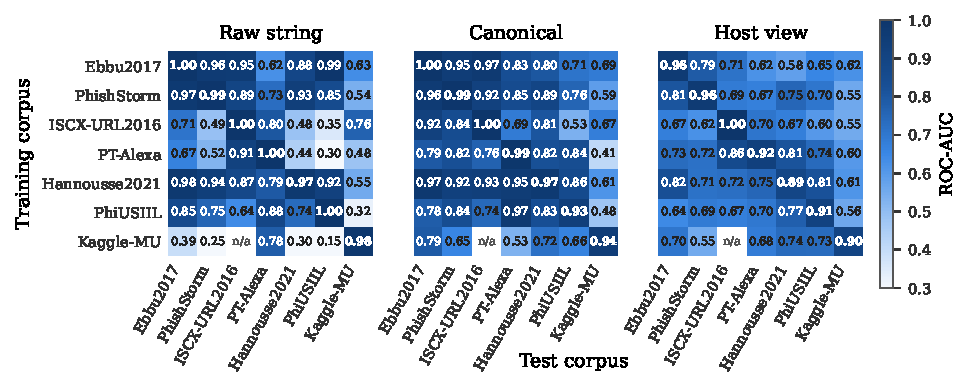
\includegraphics[width=\linewidth]{figures/fig_cross.pdf}
\caption{ROC-AUC of character n-gram models trained on one corpus (rows) and tested on another (columns), for raw strings, canonical strings and the host view. Off-diagonal cells average three seeds after removing test URLs whose canonical form occurs anywhere in the training corpus; diagonal cells (bold) are within-corpus random-split results averaged over ten seeds, without purging, and are shown for reference only. The cell marked n/a has no legitimate test URL left after purging. Darker cells are higher; the colour scale runs from 0.3 to 1.0 and values below 0.3 take the lightest colour.}
\label{fig:cross}
\end{figure}

\begin{table}[tp]
\centering
\caption{Cross-corpus transfer: ROC-AUC (MCC at threshold 0.5) averaged over the test corpora of each training corpus (five for Kaggle-MU, whose ISCX-URL2016 test set is empty after purging), and over all ordered pairs that keep both classes after purging; three seeds. Purging changes the size and class prior of a test set, which affects MCC but not ROC-AUC; per-pair sizes and priors are stored with the results. Test URLs whose canonical form occurs anywhere in the full training corpus are removed.}
\label{tab:pair_url}
\footnotesize
\begin{adjustbox}{max width=\linewidth}
\begin{tabular}{@{}lrrrrrr@{}}
\toprule
Training corpus & Pres. & Pres.+https & Lexical & Char raw & Char canon. & Char host \\
\midrule
Ebbu2017 & 0.519 (0.122) & 0.548 (-0.035) & 0.828 (0.490) & 0.840 (0.425) & 0.823 (0.487) & 0.661 (0.240) \\
PhishStorm & 0.554 (0.063) & 0.572 (0.063) & 0.771 (0.339) & 0.818 (0.481) & 0.826 (0.517) & 0.695 (0.279) \\
ISCX-URL2016 & 0.302 (-0.446) & 0.444 (-0.224) & 0.573 (-0.002) & 0.598 (0.173) & 0.744 (0.289) & 0.637 (0.153) \\
PT-Alexa & 0.506 (0.007) & 0.506 (0.007) & 0.581 (0.156) & 0.554 (0.016) & 0.741 (0.203) & 0.742 (0.346) \\
Hannousse2021 & 0.543 (0.042) & 0.589 (0.042) & 0.855 (0.567) & 0.841 (0.454) & 0.875 (0.606) & 0.739 (0.318) \\
PhiUSIIL & 0.544 (0.009) & 0.542 (0.059) & 0.623 (0.198) & 0.698 (0.083) & 0.771 (0.261) & 0.671 (0.243) \\
Kaggle-MU & 0.462 (0.191) & 0.527 (-0.024) & 0.630 (0.099) & 0.372 (0.009) & 0.670 (0.248) & 0.680 (0.253) \\
\midrule
All 41 pairs & 0.491 (-0.007) & 0.533 (-0.016) & 0.696 (0.268) & 0.682 (0.240) & 0.781 (0.376) & 0.690 (0.262) \\
\bottomrule
\end{tabular}
\end{adjustbox}
\end{table}

\begin{table}[tp]
\centering
\caption{Cross-corpus transfer: ROC-AUC (MCC at threshold 0.5) averaged over the test corpora of each training corpus (five for Kaggle-MU, whose ISCX-URL2016 test set is empty after purging), and over all ordered pairs that keep both classes after purging; three seeds. Purging changes the size and class prior of a test set, which affects MCC but not ROC-AUC; per-pair sizes and priors are stored with the results. Test URLs whose canonical form or registered domain occurs anywhere in the full training corpus are removed.}
\label{tab:pair_domain}
\footnotesize
\begin{adjustbox}{max width=\linewidth}
\begin{tabular}{@{}lrrrrrr@{}}
\toprule
Training corpus & Pres. & Pres.+https & Lexical & Char raw & Char canon. & Char host \\
\midrule
Ebbu2017 & 0.522 (0.130) & 0.551 (-0.027) & 0.822 (0.472) & 0.837 (0.413) & 0.815 (0.462) & 0.623 (0.185) \\
PhishStorm & 0.562 (0.073) & 0.577 (0.073) & 0.782 (0.350) & 0.831 (0.483) & 0.838 (0.522) & 0.679 (0.242) \\
ISCX-URL2016 & 0.300 (-0.452) & 0.444 (-0.229) & 0.575 (-0.002) & 0.595 (0.168) & 0.743 (0.285) & 0.630 (0.138) \\
PT-Alexa & 0.511 (0.024) & 0.511 (0.024) & 0.605 (0.187) & 0.533 (0.031) & 0.736 (0.214) & 0.689 (0.242) \\
Hannousse2021 & 0.546 (0.046) & 0.586 (0.046) & 0.841 (0.542) & 0.823 (0.429) & 0.864 (0.580) & 0.691 (0.253) \\
PhiUSIIL & 0.531 (-0.020) & 0.544 (0.041) & 0.636 (0.207) & 0.691 (0.080) & 0.769 (0.271) & 0.648 (0.210) \\
Kaggle-MU & 0.435 (0.192) & 0.512 (-0.038) & 0.592 (0.054) & 0.347 (-0.013) & 0.640 (0.190) & 0.638 (0.175) \\
\midrule
All 41 pairs & 0.488 (-0.006) & 0.533 (-0.015) & 0.696 (0.264) & 0.673 (0.233) & 0.775 (0.365) & 0.657 (0.207) \\
\bottomrule
\end{tabular}
\end{adjustbox}
\end{table}


Pooling six corpora does not remove corpus-specific conventions (Table~\ref{tab:loco}), and canonical input does not help everywhere. On held-out PT-Alexa the pooled raw-string model reaches an AUC of \LAUrlPTAlexaCharRaw{} and the canonical model \LAUrlPTAlexaCharCanon, while the five presentation flags alone reach \LAUrlPTAlexaPresentation. In the pooled training data almost all scheme-less strings come from Kaggle-MU, where they are somewhat more common among legitimate than among phishing URLs (Table~\ref{tab:artefacts}); the pooled probe can thus learn the direction that separates PT-Alexa, which is consistent with its high AUC. On held-out PhiUSIIL the probe with the scheme-type flag reaches \LAUrlPhiUSIILPresentationHttps, and here the raw-string model (\LAUrlPhiUSIILCharRaw) beats the canonical model (\LAUrlPhiUSIILCharCanon): the pooled raw model profits from a convention it shares with the test corpus, as in the Ebbu2017 example above. The domain purge leaves these patterns in place. ISCX-URL2016 cannot be held out, because Kaggle-MU contains every one of its legitimate URLs. On held-out Kaggle-MU every detector stays between \LAUrlKaggleMUPresentation{} and \LAUrlKaggleMUCharCanon{} AUC, which is consistent with the label inconsistencies documented in Section~\ref{sec:files} but does not prove that they cause it.

\begin{table}[tp]
\centering
\caption{Leave-one-corpus-out: ROC-AUC (MCC at 0.5) on the held-out corpus for a detector trained on the other six; three seeds. URL purge: test URLs whose canonical form occurs in any training corpus are removed; domain purge: also those whose registered domain occurs there. ISCX-URL2016 has no row because every legitimate ISCX-URL2016 URL also occurs in Kaggle-MU, so the purged test set has one class.}
\label{tab:loco}
\footnotesize
\begin{adjustbox}{max width=\linewidth}
\begin{tabular}{@{}lrrrrrr@{}}
\toprule
Held-out corpus & Pres. & Pres.+https & Lexical & Char raw & Char canon. & Char host \\
\midrule
\multicolumn{7}{@{}l}{\emph{URL purge}} \\
Ebbu2017 & 0.737 (0.385) & 0.576 (0.311) & 0.931 (0.696) & 0.986 (0.853) & 0.978 (0.831) & 0.846 (0.504) \\
PhishStorm & 0.710 (0.330) & 0.492 (0.064) & 0.850 (0.415) & 0.914 (0.473) & 0.930 (0.598) & 0.739 (0.353) \\
PT-Alexa & 0.942 (0.933) & 0.965 (0.971) & 0.947 (0.770) & 0.733 (0.037) & 0.931 (0.632) & 0.772 (0.365) \\
Hannousse2021 & 0.726 (-0.054) & 0.687 (0.436) & 0.935 (0.697) & 0.927 (0.598) & 0.957 (0.746) & 0.828 (0.411) \\
PhiUSIIL & 0.803 (0.642) & 0.988 (0.654) & 0.824 (0.619) & 0.932 (0.637) & 0.849 (0.585) & 0.772 (0.351) \\
Kaggle-MU & 0.524 (0.180) & 0.524 (0.188) & 0.578 (0.041) & 0.550 (0.087) & 0.593 (0.115) & 0.582 (0.165) \\
\midrule
\multicolumn{7}{@{}l}{\emph{Domain purge}} \\
Ebbu2017 & 0.697 (0.363) & 0.579 (0.277) & 0.918 (0.670) & 0.975 (0.800) & 0.968 (0.788) & 0.709 (0.288) \\
PhishStorm & 0.759 (0.389) & 0.478 (0.042) & 0.817 (0.330) & 0.929 (0.439) & 0.937 (0.611) & 0.718 (0.291) \\
PT-Alexa & 0.922 (0.916) & 0.946 (0.959) & 0.928 (0.722) & 0.647 (-0.046) & 0.895 (0.541) & 0.687 (0.230) \\
Hannousse2021 & 0.743 (-0.068) & 0.708 (0.403) & 0.924 (0.681) & 0.903 (0.529) & 0.934 (0.674) & 0.719 (0.248) \\
PhiUSIIL & 0.797 (0.632) & 0.987 (0.645) & 0.812 (0.607) & 0.927 (0.628) & 0.839 (0.573) & 0.760 (0.326) \\
Kaggle-MU & 0.470 (0.214) & 0.469 (0.225) & 0.558 (0.012) & 0.610 (0.071) & 0.621 (0.121) & 0.616 (0.185) \\
\bottomrule
\end{tabular}
\end{adjustbox}
\end{table}


\subsection{What the raw-string model weights}
\label{sec:ngrams}
Table~\ref{tab:ngrams} lists the n-grams with the largest weights in the raw-string model. On PT-Alexa the top phishing n-grams are fragments of \texttt{http://}. On PhiUSIIL the top legitimate n-grams are fragments of \texttt{s://www.} and the top phishing n-grams fragments of \texttt{http://}. On ISCX-URL2016 and Kaggle-MU fragments of \texttt{www.} carry phishing weight, while on PhishStorm and Hannousse2021 the same fragments carry legitimate weight. On Ebbu2017, PhishStorm and Hannousse2021 the content n-gram \texttt{.php} is among the strongest phishing features. The weights agree with the probe ablation: where a single flag separates a corpus, the raw-string model's strongest features spell that flag.

\begin{table}[tp]
\centering
\caption{Character n-grams with the largest positive (phishing) and negative (legitimate) weights in the raw-string model (seed 0, full training cap).}
\label{tab:ngrams}
\footnotesize
\begin{tabularx}{\linewidth}{@{}lXX@{}}
\toprule
Corpus & Top phishing n-grams & Top legitimate n-grams \\
\midrule
Ebbu2017 & \texttt{e/}, \texttt{php}, \texttt{.php}, \texttt{.ph}, \texttt{x/}, \texttt{hp} & \texttt{.pd}, \texttt{.pdf}, \texttt{pdf}, \texttt{e-}, \texttt{s-}, \texttt{ww} \\
PhishStorm & \texttt{php}, \texttt{hp}, \texttt{.php}, \texttt{.ph}, \texttt{.com.}, \texttt{ph} & \texttt{ww}, \texttt{://w}, \texttt{//w}, \texttt{.e}, \texttt{//www}, \texttt{://ww} \\
ISCX-URL2016 & \texttt{ww}, \texttt{/w}, \texttt{w.}, \texttt{/ww}, \texttt{/www}, \texttt{www} & \texttt{s-}, \texttt{e-}, \texttt{-t}, \texttt{a-}, \texttt{n-}, \texttt{-s} \\
PT-Alexa & \texttt{ht}, \texttt{:/}, \texttt{htt}, \texttt{http}, \texttt{ttp}, \texttt{//} & \texttt{.c}, \texttt{.com}, \texttt{.co}, \texttt{com}, \texttt{om}, \texttt{co} \\
Hannousse2021 & \texttt{php}, \texttt{.php}, \texttt{.ph}, \texttt{hp}, \texttt{pp}, \texttt{app} & \texttt{ww}, \texttt{s://w}, \texttt{//www}, \texttt{//ww}, \texttt{://ww}, \texttt{/www.} \\
PhiUSIIL & \texttt{p://w}, \texttt{p:/}, \texttt{p:}, \texttt{p://}, \texttt{ttp:}, \texttt{ttp:/} & \texttt{s://w}, \texttt{ww}, \texttt{/www.}, \texttt{www.}, \texttt{ww.}, \texttt{//www} \\
Kaggle-MU & \texttt{ww}, \texttt{www}, \texttt{www.}, \texttt{ww.}, \texttt{w.}, \texttt{://} & \texttt{.com/}, \texttt{com/}, \texttt{om/}, \texttt{m/}, \texttt{s-}, \texttt{u/} \\
\bottomrule
\end{tabularx}
\end{table}


\subsection{Does feature attribution reveal the shortcut?}
\label{sec:shap}
Phishing URL detectors are often reported with SHAP plots as evidence of what they learned \citep{mia2024}, and a security team that selects a detector with access to the model but not to the means of rebuilding its benchmark may rely on such plots. Explanation methods have known failure modes in security settings \citep{warnecke2020,nadeem2023}. We ask a narrower question: would SHAP \citep{lundberg2017} have flagged the dependence that the interventions above measure (Table~\ref{tab:shap})? Two detectors are explained on 2,000 test URLs per seed. A tree model on all 30 hand-crafted features is explained with TreeSHAP \citep{lundberg2020}, and its attribution is summed per feature group; its formatting share is the presentation flags plus the https flag, and the table lists the two apart because the scheme type can carry real signal. The raw-string n-gram model is explained with linear SHAP values, $\phi_j = w_j (x_j - \mu_j)$, which are exact on the log-odds scale when the features are treated as independent. For this model we take two per-URL shares of $|\phi|$. The own share counts n-grams that occur in a URL's raw string but not in its own canonical string. It misses n-grams absent from the URL, which also receive attribution ($-w_j \mu_j$) and carry \ShAbsentMin{} to \ShAbsentMax{} of every URL's total; a legitimate PT-Alexa entry is a bare domain equal to its canonical form, so its own share is zero by construction. The symmetric share therefore counts n-grams that are at least twice as frequent in raw as in canonical training strings, whether the URL contains them or not. Each share is set against two quantities. Drop scores the same fitted model on canonical test input and measures how much the explained model uses formatting; Loss retrains the detector without formatting and measures whether the information is needed at all.

Attribution ranks the corpora well by how much the explained model uses formatting. The rank correlation over the seven corpora between formatting share and Drop is \ShRhoTreeSame{} for the tree model ($p$ \ShRhoTreeSameP) and \ShRhoCharSymSame{} for the symmetric n-gram share ($p = \ShRhoCharSymSameP$). TreeSHAP places the largest formatting shares on PT-Alexa (\ShTreeFmtPTAlexa), PhiUSIIL (\ShTreeFmtPhiUSIIL, of which \ShHttpsPhiUSIIL{} on the https flag) and Kaggle-MU (\ShTreeFmtKaggleMU), the corpus with the largest tree Loss (\ShTreeDepKaggleMU). Against Loss, the n-gram shares still rank the corpora closely (\ShRhoChar{} for the own share and \ShRhoCharSym{} for the symmetric share, $p = \ShRhoCharP$ for both). The tree share does not ($\rho = \ShRhoTree$), but only because of PT-Alexa; without it $\rho = \ShRhoTreeNoPT$ ($p = \ShRhoTreeNoPTP$). These are descriptive figures from seven points.

What attribution does not give is the size of the loss after retraining. On PT-Alexa TreeSHAP credits \texttt{\ShTopPTAlexa} with all of the attribution, and the fitted tree fails on canonical input (Drop \ShTreeSamePTAlexa). A tree retrained without the flags loses only \ShTreeDepPTAlexa{}, because lexical features separate this corpus almost as well (MCC \WPTAlexaRandomLexical); TreeSHAP credits the feature the trees happened to split on, whether or not another feature could replace it. Ebbu2017 shows the same gap (Drop \ShTreeSameEbbu, Loss \ShTreeDepEbbu), as does the n-gram model on Hannousse2021 (Drop \ShCharSameHannousse, Loss \ShCharDepHannousse). The \texttt{has\_www} flag ranks among the three most attributed tree features on \ShWwwTopThreeN{} of the seven corpora, ISCX-URL2016 included, where the fitted tree drops by \ShTreeSameISCXURL{} on canonical input and the retrained one by \ShTreeDepISCXURL. The choice of n-gram share matters for single classes: legitimate PT-Alexa URLs move from \ShCharOwnLegitPTAlexa{} to \ShCharSymLegitPTAlexa{} under the symmetric share, and legitimate Kaggle-MU URLs from \ShCharOwnLegitKaggleMU{} to \ShCharSymLegitKaggleMU. A vocabulary-level criterion, n-grams that never occur in any canonical string, assigns at most \ShCharFmtOnlyMax{} of the attribution, because fragments such as \texttt{http} and \texttt{www} also occur inside paths and queries. The vocabularies range from \ShVocabMin{} to \ShVocabMax{} n-grams, so shares are comparable as ranks across corpora but not as levels.

A formatting-dominated attribution is thus a warning that the explained detector relies on how a corpus was recorded, a Clever Hans pattern in the sense of \citet{lapuschkin2019} and one source of the spurious correlations listed by \citet{arp2022}. Its size does not say whether a detector trained without formatting would lose anything, and a modest share is no proof that formatting is harmless; that question needs a retraining intervention such as canonicalisation.

\begin{table}[tp]
\centering
\caption{Feature attribution against two measures of dependence (random split, means over seeds 0--2, 2,000 explained test URLs per seed; MCC: Matthews correlation coefficient). Tree: gradient-boosted trees on the five presentation flags, the https flag, five structure and 19 lexical features, explained with TreeSHAP; Pres., https, Str., Lex.: shares of mean absolute SHAP value per feature group, where the formatting share used in the text is Pres.\ plus https. Char raw: the raw-string n-gram model, explained with linear SHAP (training mean as baseline, features treated as independent, log-odds scale). Own: share of a URL's $|\phi|$ on n-grams present in its raw string but absent from its own canonical string; Sym.: share on n-grams whose training document frequency in raw strings exceeds twice that in canonical strings plus five, whether present in the URL or not. Drop: MCC of the same fitted model on raw minus canonical test input. Loss: MCC of a detector retrained without formatting (the lexical model and the canonical n-gram model of Table~\ref{tab:within_random}, same seeds) subtracted from that of the explained model. Shares and MCC vary by at most 0.019 between seeds.}
\label{tab:shap}
\footnotesize
\setlength{\tabcolsep}{2.5pt}
\begin{adjustbox}{max width=\linewidth}
\begin{tabular}{@{}lrrrrrrrrrrr@{}}
\toprule
 & \multicolumn{7}{c}{Tree, 30 features (TreeSHAP)} & \multicolumn{4}{c}{Char raw (linear SHAP)} \\
\cmidrule(lr){2-8}\cmidrule(lr){9-12}
Corpus & MCC & Pres. & https & Str. & Lex. & Drop & Loss & Own & Sym. & Drop & Loss \\
\midrule
Ebbu2017 & 0.865 & 0.193 & 0.122 & 0.170 & 0.514 & 0.324 & 0.078 & 0.082 & 0.143 & 0.036 & 0.011 \\
PhishStorm & 0.818 & 0.192 & 0.003 & 0.147 & 0.659 & 0.283 & 0.063 & 0.075 & 0.116 & 0.074 & 0.005 \\
ISCX-URL2016 & 0.995 & 0.158 & 0.013 & 0.362 & 0.467 & 0.035 & 0.007 & 0.047 & 0.092 & 0.055 & $-$0.001 \\
PT-Alexa & 1.000 & 1.000 & 0.000 & 0.000 & 0.000 & 1.000 & 0.047 & 0.146 & 0.359 & 0.403 & 0.074 \\
Hannousse2021 & 0.787 & 0.180 & 0.023 & 0.132 & 0.665 & 0.136 & 0.050 & 0.133 & 0.226 & 0.246 & 0.016 \\
PhiUSIIL & 0.997 & 0.401 & 0.372 & 0.015 & 0.213 & 0.997 & 0.300 & 0.335 & 0.634 & 0.991 & 0.241 \\
Kaggle-MU & 0.892 & 0.481 & 0.011 & 0.108 & 0.401 & 0.557 & 0.328 & 0.085 & 0.162 & 0.328 & 0.144 \\
\bottomrule
\end{tabular}
\end{adjustbox}
\end{table}

